\subsection{Runtime Adaptation}
\label{sec:runtime}

At runtime, \sysname{} matches data rate to available bandwidth to minimize
latency and uses Pareto-optimal configurations to maximize accuracy.

\begin{figure}
  \centering
  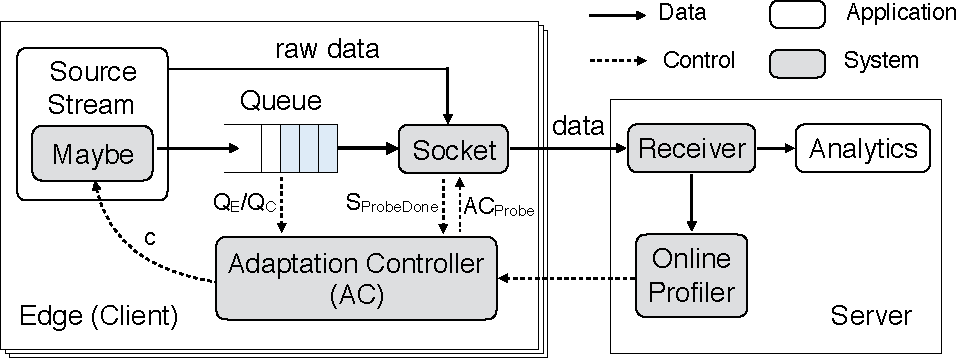
\includegraphics[width=\linewidth]{figures/runtime-adaptation.pdf}
  \caption{Runtime adaptation system architecture.}
  \label{fig:runtime}
  \vspace{-1em}
\end{figure}

\autoref{fig:runtime} shows our runtime system architecture. \sysname{}
applications' source contains a \texttt{Maybe} module derived from all \maybe{}
operators. This module allows the controller to update the level of
degradation. Data generated by the source is then enqueued to \texttt{Queue} and
subsequently dequeued by \texttt{Socket}, which sends data over the network
using TCP. When the data generation rate exceeds \texttt{Socket}'s departure
rate, the queue grows. In this case, the adaptation controller (AC) queries the
estimated bandwidth from \texttt{Socket} and regulates the source stream by
updating the configuration. After the data is sent through the network,
\texttt{Receiver} delivers data to the application analytics. \texttt{Receiver}
also performs congestion detection and extracts raw data, if it is present.  It
tracks the minimal latency (similar to how BBR tracks
\texttt{RTprop}~\cite{cardwell2017bbr} within a filter window) and reports
sudden application-level latency spikes to clients as congestion signals
(\rc{}). Raw data is only transmitted when the queue is empty and online
profiling is enabled. If a new profile is learned by the online profiler, it is
fed back to AC for subsequent adaptation.

\autoref{fig:cc-sm} shows the adaptation algorithm with a state machine model
and \autoref{fig:cc-ex} shows the state transitions with an example. We first
describe all symbols. AC loads the profile and sorts all configurations with an
ascending order of bandwidth demand, resulting in a list
$[c_1, \dots, c_{\max}]$.  These configurations follow a total order:
$c_i < c_j$ if $B(c_i) < B(c_j)$.  We denote the current configuration as $c_i$
and the next $c_{i+1}$.  AC receives messages from other modules: \qe{} when
\texttt{Queue} is empty; $\text{Q}_\text{C}$ when queued items exceed a
threshold; and \rc{} when \texttt{Receiver} detects congestion. AC can query
\texttt{Socket} for delivery rate $R$ (arrow not shown) or request it to probe
($\text{AC}_{\text{Probe}}$) for a target bandwidth, often $B(c_{i+1})$. If
there is no congestion during the probing and $R > B(c_{i+1})$, \texttt{Socket}
sends back \spd{}. Below, we describe states and transitions.

\begin{figure}
  \begin{subfigure}[t]{\columnwidth}
    \centering
    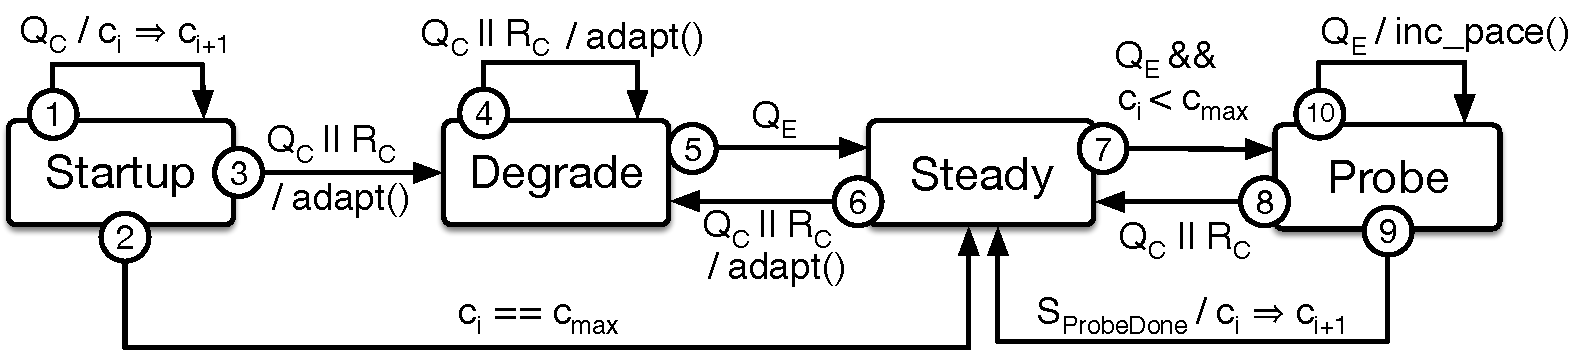
\includegraphics[width=\columnwidth]{figures/cc.pdf}
    \caption{Rate adaptation as a state machine.}
    \vspace{1em}
    \label{fig:cc-sm}
  \end{subfigure}
  \\
  \centering
  \begin{subfigure}[t]{\columnwidth}
    \centering
    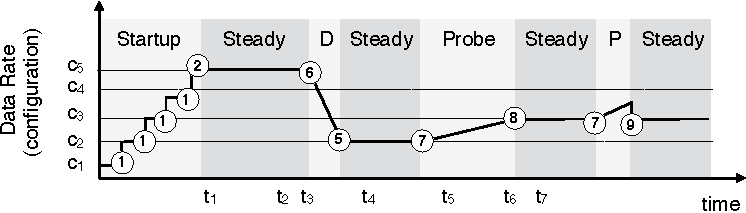
\includegraphics[width=0.9\columnwidth]{figures/cc2.pdf}
    \caption{An example illustrating the adaptation algorithm.}
    \label{fig:cc-ex}
  \end{subfigure}
  \caption{Runtime adaptation algorithm.}
  \label{fig:cc}
  \vspace{-1em}
\end{figure}

\begin{itemize}[leftmargin=*, topsep=3pt, itemsep=0pt]

\item \textbf{Startup: rapid growth.} \sysname{} starts with $c_1$ and grows the
  rate ($c_i \Rightarrow c_{i+1}$) upon each \qe{}. The growth stops at
  $c_{\max}$ (to \texttt{Steady}) or if it receives \qc{}/\rc{} (to
  \texttt{Degrade}).

\item \textbf{Degrade: reacting to congestion.} Congestion is detected in two
  ways: (1) when \texttt{Queue} grows and exceeds a threshold, AC receives
  \qc{}; (2) when \texttt{Receiver} detects latency spikes, AC receives
  \rc{}. During congestion, AC runs the \texttt{adapt()} procedure by updating
  \texttt{Maybe} with the maximum-allowed $c$ that satisfies $B(c) < \alpha R$,
  where $\alpha \in (0, 1)$ and $R$ is \texttt{Socket}'s current delivery
  rate. A smaller $\alpha$ allows a quicker draining of the queue. After the
  congestion is resolved (\qe{} received), \sysname{} changes to
  \texttt{Steady}.

\item \textbf{Steady: low latency delivery.} \sysname{} achieves low latency by
  spending most of the time in the \texttt{Steady} state. It changes to
  \texttt{Degrade} when congestion occurs. If $c < c_{\max}$ and it receives
  \qe{}, AC enters the \texttt{Probe} state to check for more available
  bandwidth.

\item \textbf{Probe: more bandwidth for a higher accuracy.} Advancing the
  configuration directly causes a drastic latency increase when
  $B(c_{i+1}) \gg B(c_i)$. To allow a smooth increase, AC requests
  \texttt{Socket} to probe by sending additional traffic controlled by
  \texttt{probe\_gain} (in \texttt{inc\_pace()}, similar to
  BBR~\cite{cardwell2017bbr}). Raw data is used for probing if available,
  otherwise we inject dummy traffic. \sysname{} stops probing under two
  conditions: (1) upon \spd{}, it advances $c_i$; (2) upon \qc{} or \rc{}, it
  returns to \texttt{Steady}.

\end{itemize}

\subsection{Resource Allocation \& Fairness}

In addition to rate adaptation, the profile is also useful for controlling a
single application's bandwidth usage or allocating resources among competing
tasks.

For individual applications, developers can pin-point a configuration for a
given bandwidth or accuracy goal. They can also specify a criterion to limit
effective configurations. For example, \sysname{} can enforce an upper bound on
the bandwidth consumption (i.e.,~do not exceed \SI{1}{Mbps}) or a lower bound on
application accuracy (i.e.,~do not fall below 50\%).

For multiple applications, their profiles allow novel bandwidth allocation
schemes such as utility fairness. Different from resource fairness with which
applications get an equal share of bandwidth, utility fairness aims to maximize
the \textit{minimal} application accuracy. With the profiles, bandwidth
allocation is equivalent to finding proper configuration $c^t$ for application
$t$. We formulate utility fairness as follows:

%% Pick one based on the space

\vspace{-0.5em}
\begin{equation}
  \vspace{-0.5em}
  \label{eq:multitask}
 \underset{c^t}{\max} \; \min({A^t(c^t)})
 \;
 \text{s.t.}
 \;
 \sum_t{B^t(c^t)} < R
\end{equation}

% \begin{equation}
%  \label{eq:multitask}
%  \begin{aligned}
%     & \underset{c^t}{\text{maximize}} & & \min({A^t(c^t)}) & & \\
%     & \text{subject to} & & \sum_t{B^t(c^t)} < R & & \\
%  \end{aligned}
% \end{equation}

Solving this optimization is computationally hard. \sysname{} uses heuristics
similar to VideoStorm~\cite{zhang2017live}: it starts with $c^t_1$ and improves
the application $t$ with the worst accuracy; this process iterates until all
bandwidth is allocated.

%%% Local Variables:
%%% mode: latex
%%% TeX-master: "../awstream"
%%% End:

%% LocalWords: runtime analytics enqueued dequeued TCP JetStream
%% LocalWords: RTprop BBR profiler sm VideoStorm